%
\chapter{Določanje smeri s kompasi}
\label{Ch_Kompasi} % use \chaptermark{}
% to alter or adjust the chapter heading in the running head

Kompasi so navigacijske priprave za določanje smeri v prostoru. Prostor definira koordinatni sistem, ki ga izberemo kot operaterji.

V izbranem koordinatnem sistemu definiramo izhodišče, smer (dve ali tri, odvisno od zahtev) in merilo. Med navigacijo v prostoru določamo smeri: ali vektor lastnega gibanja ali vektor pogleda in zanj definiramo koordinatni sistem v katerem bomo to počeli. Na izbiro imamo kartezični, polarni ali krogelni koordinatni sistem. Odločamo se za sistem, v katerem je zapis vektorja najbolj naraven oz. najlažje razumljiv. Vzemimo za primer radar: zaradi varnosti plovbe bodo opisi vektorjev gibanja okoliških plovil  najbolj razumljivi, ko bo v izhodišču naše plovilo. Za zapise relativnih oddaljenosti uporabljamo polarni sistem, v katerem vsak objekt ponazorimo z oddaljenostjo in azimutom od izhodišča. V vesoljski navigaciji po našem Osončju je izhodišče v središču Sonca, v ladijski navigaciji se tradicionalno odločamo za tri dimenzijski koordinatni sistem z izhodiščem v središču Zemlje. Vozila in plovila značilno uporabljajo tudi svoj lastni koordinatni sistem, z izhodiščem v svojem lastnem masnem središču. 

Od metod za določanje smeri v prostoru sta uporaba magnetnega in vrtavčnega kompasa le dve od številnih možnosti.  

%https://www.nature.com/articles/s41467-017-00059-9 Za vrtavčne kompase se uporabljajo trajni magneti: Structure and behavior of permanent magnets on the atomic level
%(Nanowerk News) Scientists at TU Darmstadt explored on an atomic level how changes in iron content influence the micro-structure of samarium-cobalt based permanent magnets. Their results were published in Nature Communications ("Atomic structure and domain wall pinning in samarium-cobalt based permanent magnets"). In the long run they could contribute to the development of permanent magnets with improved magnetic performance. These magnets can be found in microwave tubes, gyroscopes and satellite controls, for instance.
%Although samarium cobalt magnets (Sm2Co17 magnets), a type of rare earth permanent magnets, were developed in the early 1960’s the underlying domain wall pinning mechanism has remained unknown. Scientists at TU Darmstadt showed that the iron content controls the formation of a diamond-shaped cellular structure that dominates the density and strength of the domain wall pinning sites and thus the coercivity, in other words the resistance the magnet puts up against demagnetization.
%Read more: Structure and behavior of permanent magnets on the atomic level 

%AutoComp 1000 https://www.kvh.com/Commercial-and-OEM/Gyros-and-Inertial-Systems-and-Compasses/Compass-Sensors/All-Compass-Sensors-Systems/AutoComp-1000.aspx
%Autocomp 1000
%PRODUCT IMAGES:  Previous ImageNext Image
%The AutoComp 1000 employs KVH’s breakthrough digital fluxgate compass technology to provide precision heading data to an array of systems, including autopilots, GPS, video charts, radars, computers, and other electronic instruments.
%
%Designed as a remote sensor, the AutoComp 1000 can be mounted in a magnetically “clean” location (e.g., away from speakers, motors, wiring bundles, and other sources of changing magnetic fields), and its continuous automatic compensation feature ensures that the most precise heading data (within ±0.5°) is available at all times. The AutoComp 1000 is fully compatible with the NMEA 0183 output standard and a universal interface card is available for use with other interface standards. 
%Highlights
%Remote sensor with continuous autocompensation ensures reliable heading data at all times
%Accurate to within ±0.5°
%Fast 10 Hz NMEA 0183 standard output compatible with ARPA radars, autopilots, and other electronic systems; optional interface card available for other outputs
%


\begin{table}
	\centering
	\caption{Pregled tipal za določanje smeri in njihovih značilnosti}
	\label{tabKomp}       % Give a unique label
    \resizebox{11cm}{!} 
{
\begin{tabular}{|p{3cm}|p{4cm}|p{3,5cm}|p{3cm}|}
	\hline 
	vrsta tipala & vrsta meritve & omejitve & točnost \\ 
	\hline 
	sledilnik zvezd & triosna usmerjenost z vektorskimi meritvami večih zvezd & vidnost zvezd & 1 kotna sekunda \\ 
	\hline 
	običajni Sončni senzor & vektor proti Soncu & vidnost Sonca & 1 kotna minuta \\ 
	\hline 
	magnetometer & vektor vzdolž silnic magnetnega polja & prisotnost magnetnega polja & 0,5\degree \\ 
	\hline 
	žiroskop & inercijska sprememba triosne usmerjenosti &  & relativna meritev kota \\ 
	\hline 
	GNSS & triosna usmerjenost z meritvami do večih satelitov & zadosten sprejem signalov satelitov & 0,1\degree, glede na geometrijo in večžarkovni prenos \\ 
	\hline 
	senzor obzorja & vektor proti središču Zemlje & obzorje mora biti vidno & 0,1\degree \\ 
	\hline 
	pospeškometer in inklinometer & vektor proti središču Zemlje & mora biti v težnostnem polju Zemlje, ne deluje v vesolju & 0,1\degree \\ 
	\hline 
	triosni Sončni senzor  & triosna usmerjenost glede na vektor proti Soncu in vrtilno os Sonca & vidnost Sonca & 0,1\degree \\ 
	\hline 
\end{tabular} 
}
\end{table}

%SEPTEMBER 13, 2016 TOO MUCH MAGNETISM: http://www.hsisensing.com/too-much-magnetism/

V čem je osnovni trik, ko uporabljamo kompas? Vedeti moramo, kako je trenutno kazanje kompasa usklajeno s smermi, ki jih lahko najdemo na navigacijski karti. Če bi radi na karti določili smer našega trenutnega pogleda, odčitamo (na primer s pomočjo smerne plošče) s kompasa za koliko stopinj smer našega pogleda odstopa od izhodiščne smeri. Referenciranje je izvedeno na neko točko v prostoru, prostor je definiran z njegovimi koordinatnimi osmi.

Sodobni digitalni magnetometri so nepremični potomci klasičnih kompasov z gibljivo magnetno iglo. Vsebujejo tri tipala magnetnega polja, vsak je obrnjen vzdolž svoje osi kartezičnega koordinatnega sistema. Vzemimo, da magnetometrova smer x usmerjena v smeri plovbe (naprej), y bočno v levo in z navpično navzgor. Če je trenutno premec našega plovila na mirnem morju obrnjen v smer lokalnega geomagnetnega meridiana, bo naš digitalni kompas določil praktično samo komponento x, medtem ko bosta y in z enaki nič. Z razmerjem velikosti treh komponent magnetnega polja se torej lahko orientiramo glede na lokalni geomagnetni meridian. 

Zakaj pravimo \textit{praktično} in ne \textit{popolnoma}? V idealnem primeru bi magnetni kompas kazal smer geomagnetnega meridiana. V realnosti moramo upoštevati, da na določitev kurza z magnetnim kompasom vpliva tudi napaka, ki jo imenujemo magnetna deviacija. Magnetno deviacijo določa magnetizem plovila in jo moramo poznati. Vedeti moramo, da magnetizem plovila določajo v njegovo konstrukcijo opločja on gredi vgrajene trdomagnetne snovi, ki povzročajo trajni magnetizem plovila in mehkomagnetne snovi, ki povzročajo prehodni magnetizem plovila. Med obračanjem ladje se namreč vpliva obeh magnetizmov na kazanje magnetnega kompasa spreminjata, kar ponazarja t.i. deviacijska krivulja.

Če deviacijsko krivuljo zapišemo s trigonometrijsko vrsto, s katero upoštevamo vse vplive omenjenih magnetizmov, vrsta vsebuje neskončno število členov. Nekatere člene v približni formuli deviacije zanemarimo, ker so njihovi vplivi na obliko krivulje zanemarljivi.

Smisel kompenzacije vpliva določenega prehodnega magnetnega polja na magnetno rožo ladijskega kompasa je zmanjšanje amplitude deviacijske krivulje in s tem v kompasu z gibljivimi deli povečanje momenta vrnitve.

Kako pa zmanjšujemo vplive magnetizma konstrukcije na trgovskih ladjah? Na trgovskih ladjah kompenziramo: vzdolžno komponento B trajnega magnetizma (z vzdolžnimi magneti), komponento C (s prečnimi magneti), komponento D (s kroglama), od prehodnega pa vplive parametrov -a in -e, ter parameter -c (s Flindersovo palico), ostalih vplivov pa ne kompenziramo.

V praksi na kazanje magnetnega kompasa vplivata poleg magnetizma opločja ladje tudi vsa oprema in tovor. 


Naloga:

Narišite graf deviacijske krivulje za vse kompasne kurze ($K_k$), če so podani približni koeficienti: A = – 0,5\degree, B = +21\degree, C = – 4\degree, D = + 3,7\degree, E = + 0,5\degree! Deviacijo podajte v razpredelnici, tako da v vrsticah navedete podane vrednosti koeficientov od A do E, v stolpec pa kardinalne in interkardinalne $K_k$!

Rešitev:

Neodvisna spremenljivka (argument) funkcije deviacije je kompasni kurz $K_k$. 
$$
\delta = A + B sin(K_k) + C cos(K_k) + D sin(2 K_k) + E cos(2 K_k)
$$


% For tables use
%
\begin{table}
	\centering
	\caption{V obliki tabele smo izračunali prispevke členov trigonometrijske vrste. Člene določajo koeficienti in kompasni kurz Kk, ki smo ga vzeli pod drobnogled le v kardinalnih in interkardinalnih smereh. Rezultat je viden na krivulji slike \ref{Fig_PrimerDeviacijskeKrivulje}}
	\label{TabMagDev}       % Give a unique label
	%
	% For LaTeX tables use
	%
	\begin{tabular}{lccccccc}
		\hline\noalign{\smallskip}
		smer & $K_k$  & člen A & člen B & člen C & člen D & člen E & $\delta$ \\
		N & 0\degree & -0.5\degree & 0.0\degree & -4.0\degree & 0.0\degree & 0.5\degree & -4.0\degree \\
		NE & 45\degree & -0.5\degree & 14.8\degree & -2.8\degree & 3.7\degree & 0.0\degree & 15.2\degree \\
		E & 90\degree & -0.5\degree & 21.0\degree & 0.0\degree & 0.0\degree & -0.5\degree & 20.0\degree \\
		SE & 135\degree & -0.5\degree & 14.8\degree & 2.8\degree & -3.7\degree & 0.0\degree & 13.5\degree \\
		S & 180\degree & -0.5\degree & 0.0\degree & 4.0\degree & 0.0\degree & 0.5\degree & 4.0\degree \\
		SW & 225\degree & -0.5\degree & -14.8\degree & 2.8\degree & 3.7\degree & 0.0\degree & -8.8\degree \\
		W & 270\degree & -0.5\degree & -21.0\degree & 0.0\degree & 0.0\degree & -0.5\degree & -22.0\degree \\
		NW & 315\degree & -0.5\degree & -14.8\degree & -2.8\degree & -3.7\degree & 0.0\degree & -21.9\degree \\		
		\noalign{\smallskip}\hline
	\end{tabular}
\end{table}



\begin{figure}[!ht]%{0.5\textwidth}
	\vspace{0pt}
	\begin{center}
		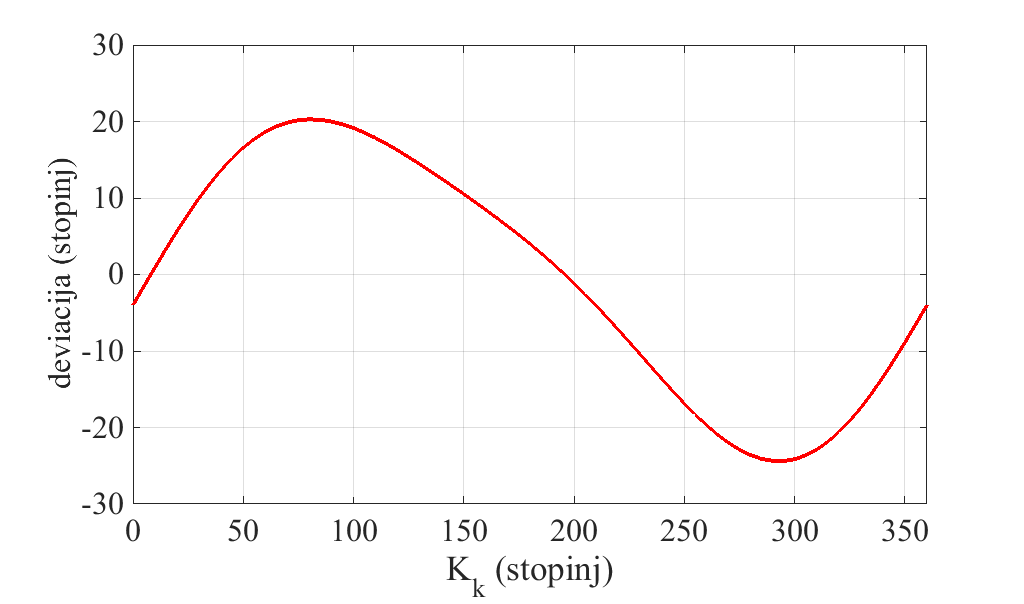
\includegraphics[width=0.65\textwidth]{Predavanja/02_KompasnoDolocSmeri/figs/DeviacijaPoPriblFormuli.png}
	\end{center}
	\vspace{0pt}
	\caption{Prikaz deviacijske krivulje $\delta(K_k) $ za dane vrednosti koeficientov A, B, C, D in E.}
	\label{Fig_PrimerDeviacijskeKrivulje}
	\vspace{0pt}
\end{figure}
   

Če pa nosimo pameten magnetometer s seboj in vemo, da se v bližini nahaja močan izvor magnetnega polja, nam pameten kompas spet z razmerji velikosti treh komponent ne le kaže smer do njega, ampak s pomočjo merjenja rezultante gostote magnetnega pretoka lahko ocenjujemo ali se magnetnemu izvoru (magnetnemu polu) približujemo ali se od njega oddaljujemo.

%https://www.javad.com/jgnss/javad/news/pr20160717.html

Pri določanju smeri in ocenjevanju oddaljenosti od objekta se moramo zavedati, da so v prostoru tudi objekti, ki nas pri tem iskanju ne zanimajo, zato moramo njihov vpliv odmisliti. Za odpravljanje njihovega vpliva ali na iskanje ali vsaj določanje smeri do izbranega izvora, moramo poznati 'magnetni podpis' nezanimivih objektov. 

Ladijski navigator, ki določa zasuk kurza svoje ladje od magnetnega meridiana, mora imeti verodostojen zgoščen popis podpisov vseh magnetno motečih objektov oz. njihovih vplivov na kazanje magnetnega kompasa - temu popisu rečemo deviacijska krivulja. Z odštetjem magnetne deviacijske krivulje od izmerjene vrednost magnetnega polja s kompasom dobi navigator smer meridiana geomagnetnega polja v katerem je ladja v trenutku meritve ladja. Z znano deviacijo torej določimo magnetni kurz ladje.  

\subsection{Magnetna deklinacija oz. variacija}

Za določitev \textit{magnetnega} kurza moramo natančno določiti zasuk smeri premca ladje od magnetnega meridiana $N_{mm}$. Upoštevati moramo magnetno deviacijo (glej primer na sliki \ref{Fig_PrimerDeviacijskeKrivulje}), ki kot preverljiva sistematična napaka za znano vrednost suka odčitek kompasa $K_k$ od magnetnega kurza $K_m$. 

Za določitev \textit{pravega} kurza plovbe pa moramo poznati variacijo. Pri navigaciji nas sploh ne zanima relativna smer do nobenega magnetnega pola, saj sta ponavadi predaleč oz. ker med njima ne poteka ravna, ampak nepravilno vijugasta krivulja, vzdolž katere je magnetna deklinacija enaka. Magnetni meridiani so tangente na te krivulje enake magnetne deklinacije (glej sliko \ref{Fig_KartaVariacije}). Geografi namreč na vsako pomorsko navigacijsko karto, ki prikazuje izsek iz svetovne karte, vrisujejo podatek o lokalni magnetni variaciji, ki mora zadosti dobro veljati za celotno območje navigacijske karte, tako v njenem središču, kot na robovih. Vrednosti lokalne variacije ob času nastanka karte je na karti dodana tudi hitrost spreminjanja variacije s časom. Upoštevanje lokalne variacije, ki torej ponazarja smer lokalnega magnetnega meridiana, v katero naj bi kazala magnetna igla, če ladja na bi bila magnetna in če kompas ne bi imel lastne napake (kot vsak merilni instrument), nam omogoča določiti pravi kurz ladje.


\begin{figure}[!ht]%{0.5\textwidth}
	%\vspace{0pt}
	\begin{center}
		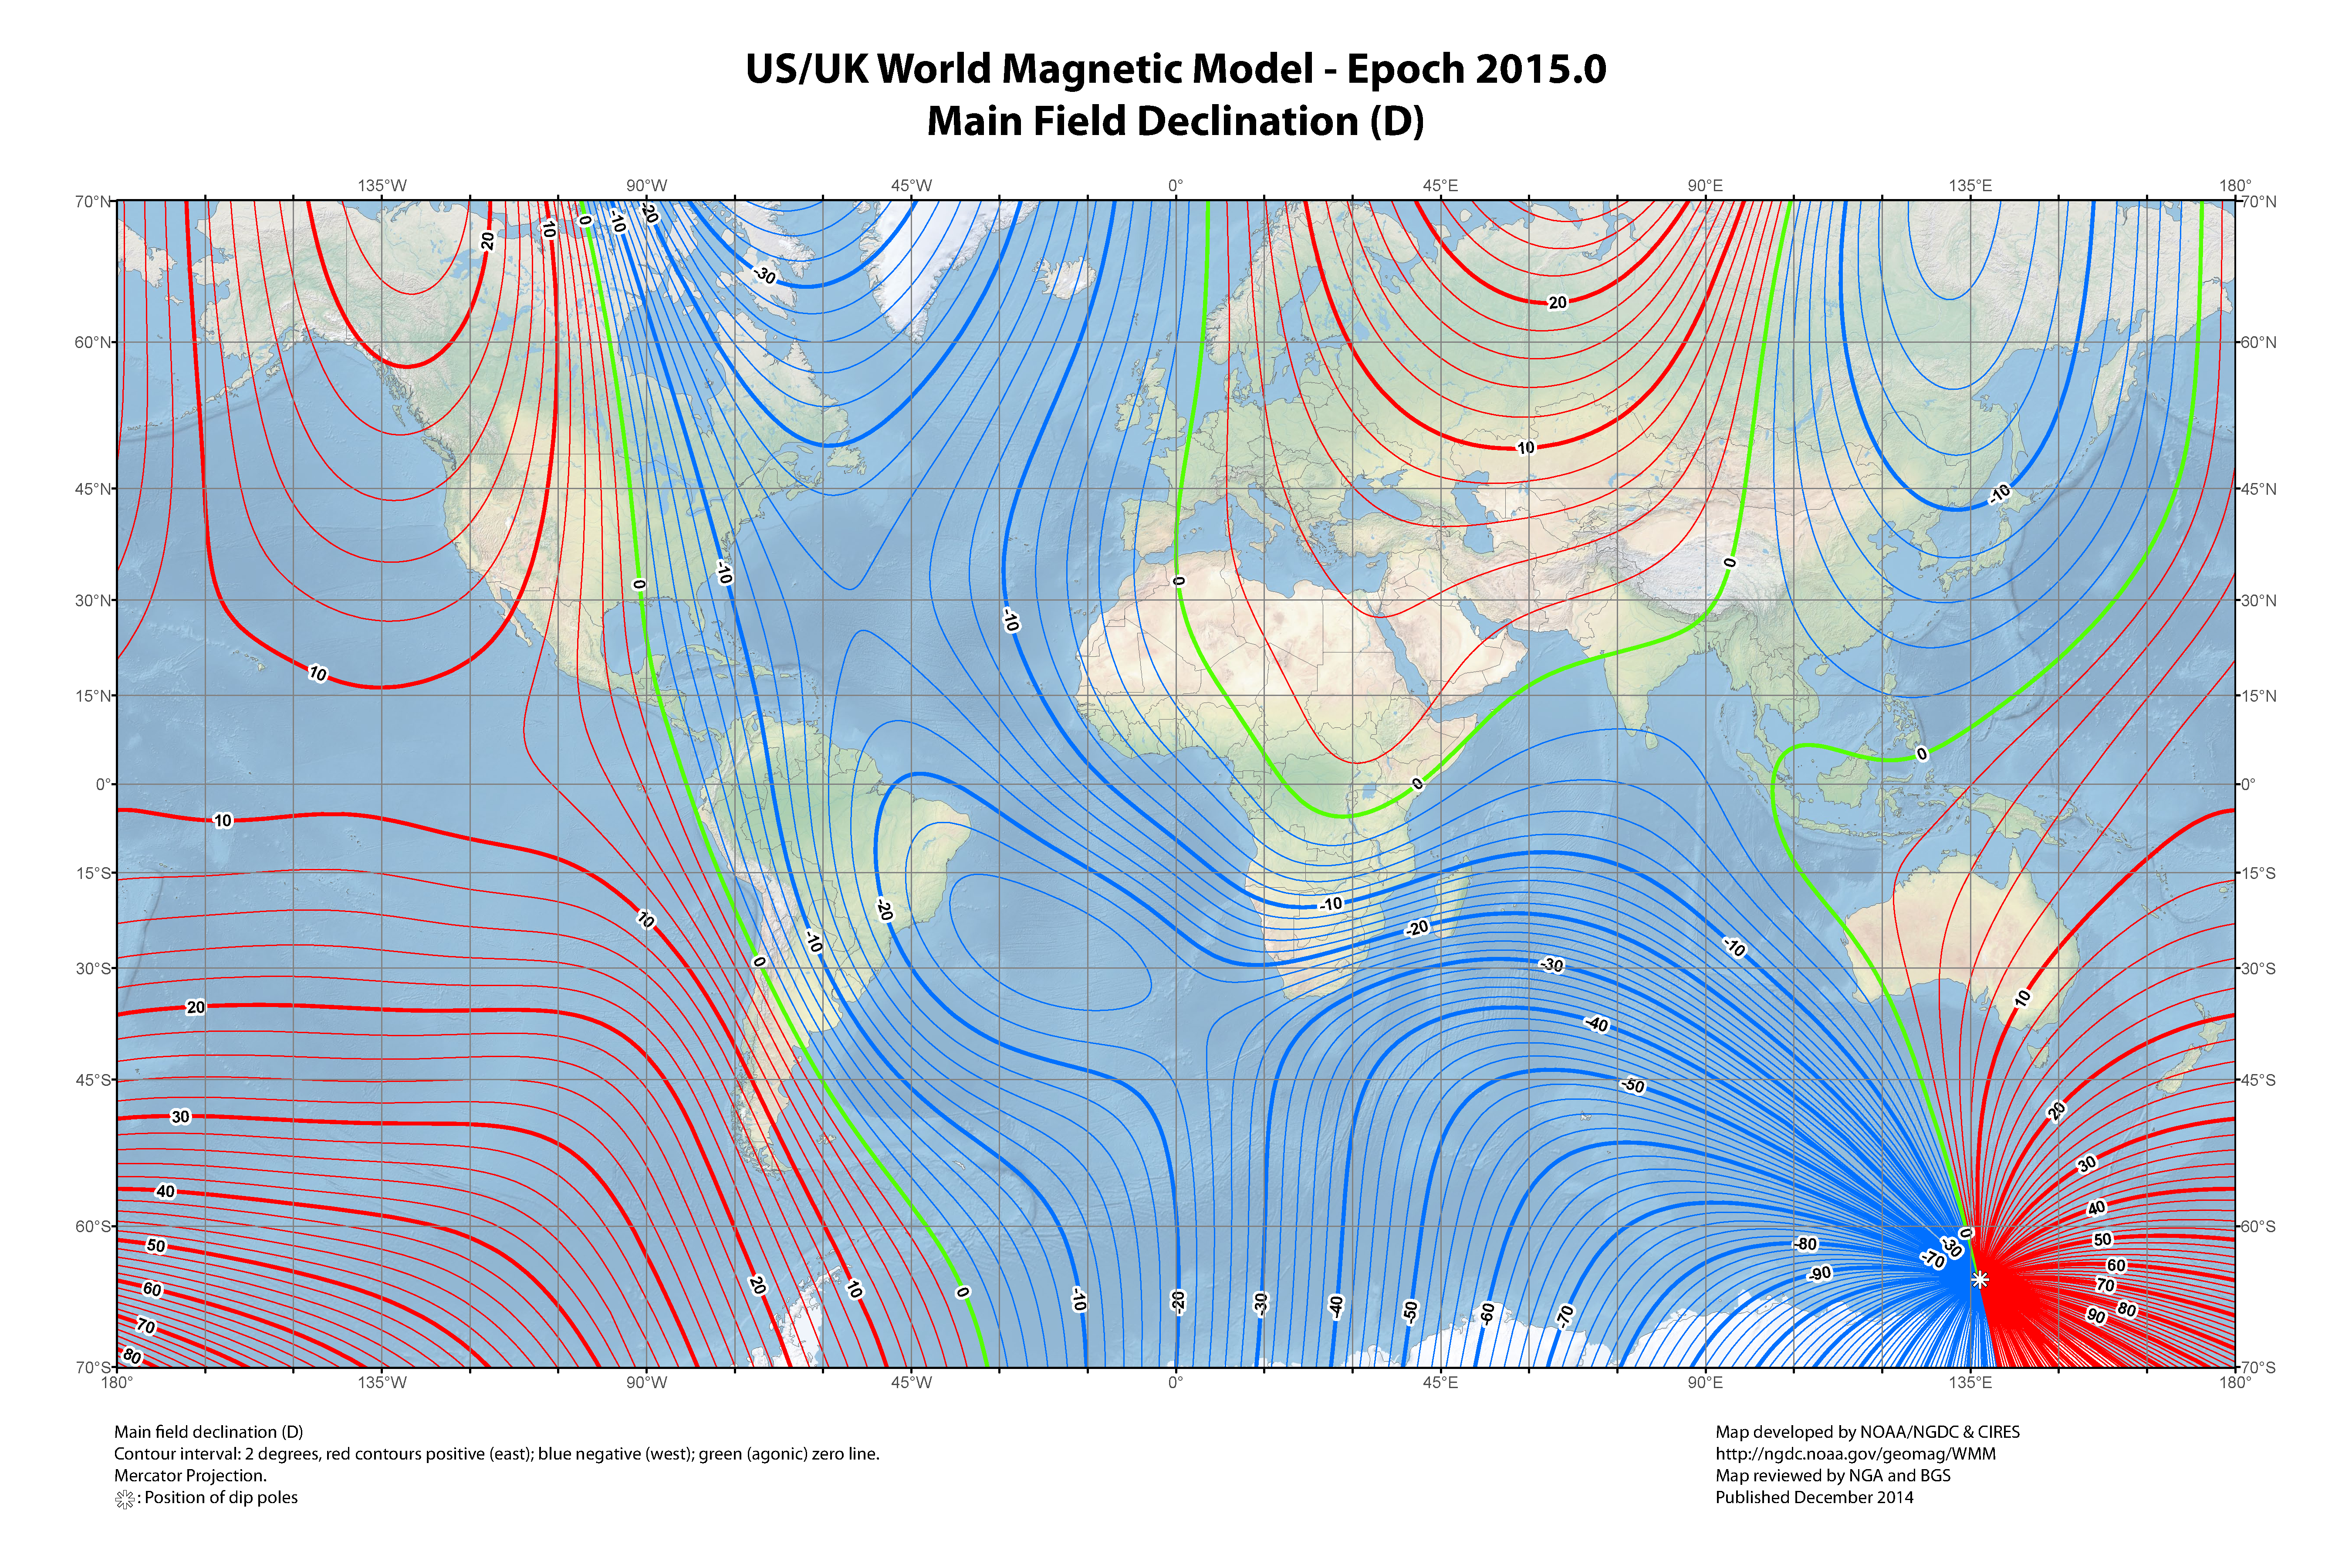
\includegraphics[width=0.65\textwidth]{Predavanja/02_KompasnoDolocSmeri/figs/WMM2015_D_MERC.pdf}
	\end{center}
	%\vspace{0pt}
	\caption{Svetovna karta magnetne deklinacije oz. variacije, podane v Mercatorjevi projekciji, je pripomoček, za določanje magnetnih meridianov področij, ki jih zajemajo posamezne navigacijske karte.\cite{WorldMagModel}.}
	\label{Fig_KartaVariacije}
	\vspace{0pt}
\end{figure}

%http://geokov.com/education/magnetic-declination-inclination.aspx


\begin{figure}[!ht]%{0.5\textwidth}
	\vspace{0pt}
	\begin{center}
		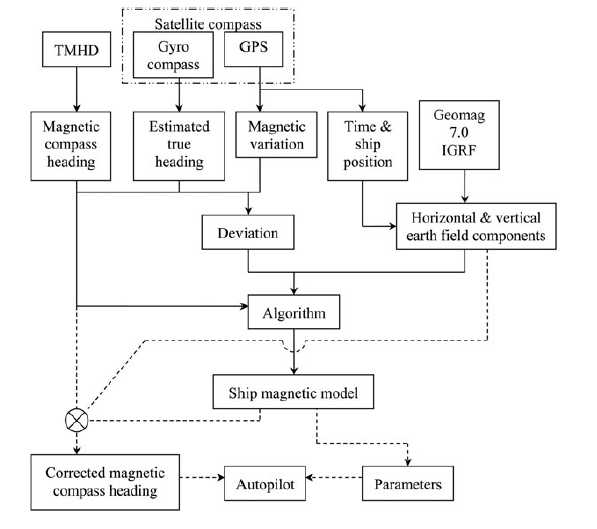
\includegraphics[width=0.65\textwidth]{Predavanja/02_KompasnoDolocSmeri/figs/2016AlgoritemKorigiranjaKompasa.png}
	\end{center}
	\vspace{0pt}
	\caption{Prikaz algoritma korigiranja kazanja, \cite{Basterr}.}
	\label{Fig_KorigiranjeKompasaMedPlovbo}
	\vspace{0pt}
\end{figure}

Umerjanje kompasov?

\begin{figure}[!ht]%{0.5\textwidth}
	\vspace{0pt}
	\begin{center}
		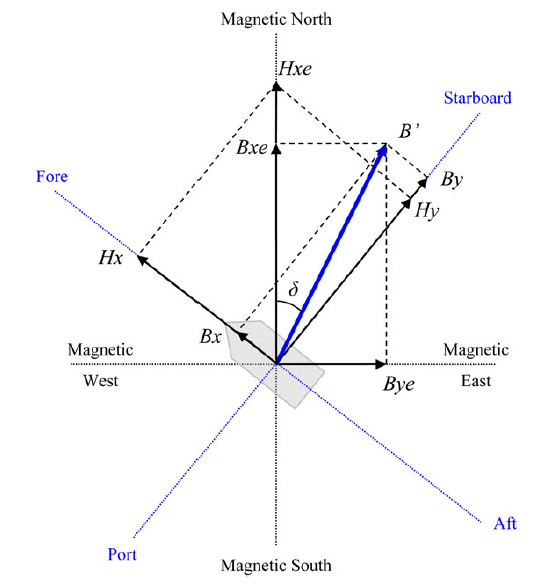
\includegraphics[width=0.48\textwidth]{Predavanja/02_KompasnoDolocSmeri/figs/2016LadijskiMagnetniVektorji.png}
	\end{center}
	\vspace{0pt}
	\caption{Prikaz vektorjev magnetnih veličin za opis ladijskega in zemeljskega magnetizma. \cite{Basterr}}
	\label{Fig_LadijskiMagnetniVektorji}
	\vspace{0pt}
\end{figure}

% THE JOURNAL OF NAVIGATION (2016), 69, 1325–1340. © The Royal Institute of Navigation 2016 doi:10.1017/S0373463316000138
%Towards an Improvement of Magnetic Compass Accuracy and Adjustment
%Imanol Basterretxea-Iribar, Iranzu Sotés and Jose Ignacio Uriarte
%(E.T.S. de Náutica y Máquinas Navales, University of the Basque Country, UPV/EHU, Portugalete, Bizkaia, Spain)
%(E-mail: imanol.basterrechea@ehu.es)
%Many ship accidents have arisen from an error in course indication. Bearing in mind that the actual errors in gyrocompass and satellite compass are really minor, they may be considered valid to be input into an autopilot provided that any failure in such devices is controlled by means of a secondary heading source such as a magnetic compass. However, magnetic compass deviation may be significant and its heading should be corrected before being input to the autopilot. The errors caused by the geographic variability of the deviation
%should also be taken into account. Moreover, the current way to reduce the deviation requires that the ship is un-berthed to execute a complete swing. The aim of this article is to obtain a ship magnetic model by means of an algorithm based on least squares to correct magnetic compass heading input in the autopilot and to permit definitive magnetic compass compensation without swinging the ship through 360°.


Risanje zemljevidov (map) in navigacijskih kart?

%'maps are to be looked at, charts are to be worked on'. Mercator’s world map of 1569 was useless for navigation at the time it was created because navigation was something different from his idealised concept. (Joaquim Alves Gaspar, REVISITING THE MERCATOR WORLD MAP OF 1569, an Assessment of Navigational Accuracy, THE JOURNAL OF NAVIGATION (2016), 69, 1183–1196. © The Royal Institute of Navigation 2016, doi:10.1017/S0373463316000291)
%
%Merkatorjeva karta iz leta 1569 je bila neuporabna za navigacijo:
%'The reason is that courses were measured relative to the magnetic north, not to the geographical north. In order to convert compass courses into geographic courses and vice versa one would need to know the value of magnetic declination in the area of interest.'
%
%Če pa bi poznali variacijo/deklinacijo za vsako točko:
%'Suppose that this difficulty was solved by carrying out a systematic survey of the magnetic declination in the Atlantic. Assuming that the charts were free of any other errors, would this improvement allow the pilots to effectively use the Mercator projection? Yes, on the condition that all magnetic courses measured with the marine compass were corrected before being transferred to the chart and that the geographic courses retrieved from the chart were converted to magnetic courses before being used to steer the ship. However this hypothetical situation could not be met at the time Mercator proposed his projection: no accurate Mercator chart existed and none could be constructed because the longitudes of the places were not known with the necessary accuracy'
%
%That was the case of all pre-Mercator nautical charts, which were constructed on the basis of magnetic courses, estimated distances and, from about 1500 on, the latitudes of the places. This is a different paradigm from the one adopted by Mercator in his world map, which was constructed on the basis of the latitudes, longitudes and true geographic directions. The critical point to note is that the two cartographic models – the pre-Mercator chart and the Mercator projection – are different and hardly compatible with each other in so far as the practice of navigation is concerned. Even if the latitudes and longitudes in Mercator’s world map were accurate (which is not the case), it could not have been used to support navigation at the time it was proposed. The reason is that courses were measured relative to the magnetic north, not to the geographical north. In order to convert compass courses into geographic courses and vice versa one would need to know the value of magnetic declination in the area of interest



\section{Sodobni kompasi}
\label{PogKompSod}
% Always give a unique label
% and use \ref{<label>} for cross-references
% and \cite{<label>} for bibliographic references
% use \sectionmark{}
% to alter or adjust the section heading in the running head
FOG

\subsection{Pretočni kompas}
\label{PopdpPretKomp}
Your text goes here.

\begin{equation}
	\vec{a}\times\vec{b}=\vec{c}
\end{equation}

\subsubsection{Subsubsection Heading}
Your text goes here. Use the \LaTeX\ automatism for cross-references as
well as for your citations, see Sect.~\ref{sec:1}.

\paragraph{Paragraph Heading} %
Your text goes here.

\subparagraph{Subparagraph Heading.} Your text goes here.%
%
\index{paragraph}
% Use the \index{} command to code your index words
%
%
%
% For figures use
%
\begin{figure}[!ht]%{0.5\textwidth}
	\vspace{0pt}
	\begin{center}
		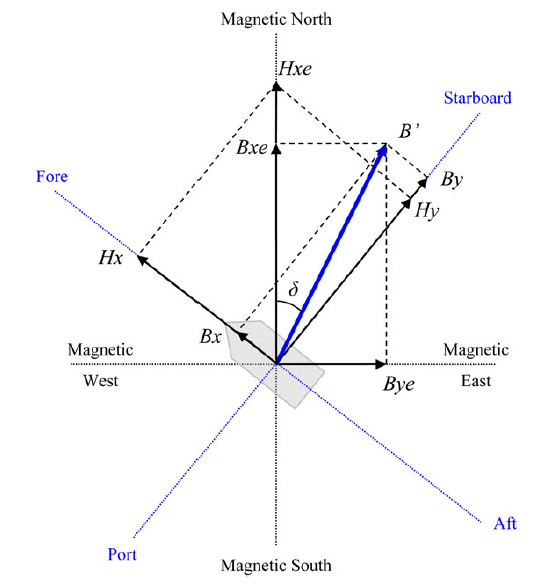
\includegraphics[width=0.48\textwidth]{Predavanja/02_KompasnoDolocSmeri/figs/2016LadijskiMagnetniVektorji.png}
	\end{center}
	\vspace{0pt}
	\caption{Prikaz vektorjev magnetnih veličin za opis ladijskega in zemeljskega magnetizma. \cite{Basterr}}
	\label{Fig_LadijskiMagnetniVektorji}
	\vspace{0pt}
\end{figure}
%
% For built-in environments use
%
\begin{theorem}
	Theorem text goes here.
\end{theorem}
%
% or
%
\begin{lemma}
	Lemma text goes here.
\end{lemma}
%
%
% Problems or Exercises should be sorted chapterwise
\section*{Problemi}
\addcontentsline{toc}{section}{Problemi}
%
% Use the following environment.
% Don't forget to label each problem;
% the label is needed for the solutions' environment
\begin{prob}
	\label{prob1}
	Problem določanja pravega kurza, če poznamo \textbf{prave vrednosti}: kompasni kurz, variacijo, .. %(H:\DVD_Groves\Examples\Example_6_1) 
\end{prob}

\begin{prob}
	\label{prob2}
	\textbf{Problem Heading}\\
	(a) The first part of the problem is described here.\\
	(b) The second part of the problem is described here.
\end{prob}



%
